\begin{figure}[h]
	\centering
	\begin{minipage}{.45\textwidth}
		\centering
		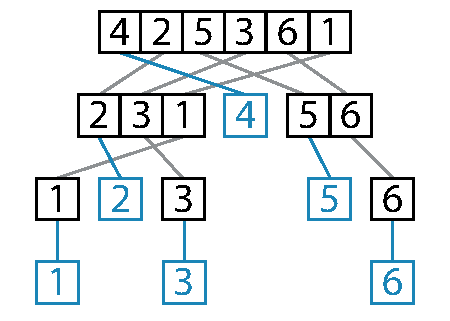
\includegraphics[width=\textwidth]{Graphics/Quicksort_example_avg}
	\end{minipage}
	\begin{minipage}{.45\textwidth}
		\centering
		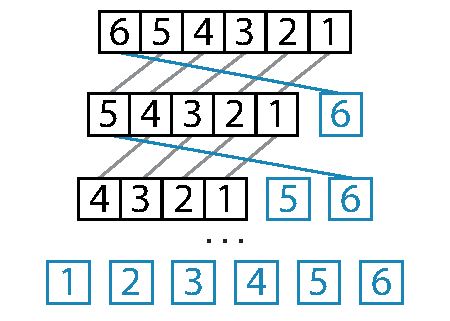
\includegraphics[width=\textwidth]{Graphics/Quicksort_example_wcet}
	\end{minipage}
	\caption{Beispiel für durchschnittliche(links) und schlechteste(rechts) Ausführungszeit eines primitiven Quicksort}
	\label{fig:quicksort_example}
\end{figure}

\paragraph{Beobachtung:}
Die Laufzeit des Quicksort-Algorithmus hängt maßgeblich von der Wahl des Pivotelements ab:
\begin{itemize}
	\item \textbf{Best-Case:} Das Pivotelement wird so gewählt, dass gilt $||L| - |R| | \leq 1$. Daraus ergibt sich mit $log(n)$ Schritten mit je $n$ Vergleichen eine Laufzeit von $\mathcal{O}(nlog(n))$.
	\item \textbf{Worst-Case:} Das Pivotelement wird so gewählt, dass gilt $|L| = 1$ oder $|R| = 1$. Daraus ergibt sich mit $n$ Schritten und je $n$ Vergleichen eine Laufzeit von $\mathcal{O}(n^2)$.
\end{itemize}